% Section 3: Illustrative example
\section{Illustrative example}
\label{sec:illustrative-example}

This section evaluates FHOPS on the public British Columbia ground-based ladder (tiny7, small21, med42) plus synthetic scaling tiers. In this ladder, horizons increase from 7 to 21 to 42 days and block counts from 2 to 6 to 12 with the same 9-machine role mix. The goal is a reproducible baseline for practitioner interpretation and follow-on modelling studies, consistent with review-identified reproducibility gaps \cite{jaffray2025systematic}.

We organize the results around three operational questions:
\begin{enumerate}
  \item What quality-runtime trade-offs are observed across solver families?
  \item How robust are resulting schedules under operational disturbances?
  \item What cost and scale signals are visible from the current baseline?
\end{enumerate}

\subsection{Operational question 1: quality-runtime trade-offs across solver families}
Table~\ref{tab:benchmarks} summarizes SA, ILS, and Tabu outcomes by scenario. Three patterns are relevant for planning decisions.
\begin{itemize}
  \item \textbf{Small instance (tiny7):} objectives are tightly grouped (4306.52--4349.26) and production is identical (4414.70~m$^3$), while runtime spans 32.71--292.53~s.
  \item \textbf{Intermediate instance (small21):} objective spread remains narrow (15627.57--15660.01) with identical production (15966.97~m$^3$), but runtime spans 77.94--414.78~s and mobilisation cost spans 1924.56--2243.76~CAD.
  \item \textbf{Larger instance in this ladder (med42):} KPI ordering is not uniform across objective, production, and runtime (objective: $-28271.22$ to $-46063.73$; production: 30026.28--32702.07~m$^3$; runtime: 124.48--182.33~s), so solver selection should follow planning priorities rather than one headline score.
\end{itemize}

Table~\ref{tab:tuning} adds parameter-search evidence. Reported $\Delta$ values versus the SA default are 42.74 (tiny7), 10.23 (small21), 11454.66 (med42), and 0.00 (synthetic-small), showing scenario-dependent tuning impact. Controlled tuning can therefore improve schedules without changing the underlying data contract \cite{nelson2003forestmodels}.

\begin{table}[t]
  \centering
  \caption{Solver performance across the reference scenarios. Objective values are compared within scenario (not across scenarios) because sign and scaling differ by dataset/weight profile.}
  \label{tab:benchmarks}
  \input{sections/includes/solver_performance.tex}
\end{table}

\begin{table}[t]
  \centering
  \caption{Best-performing tuner per scenario (delta measured against SA's default preset).}
  \label{tab:tuning}
  \input{sections/includes/tuning_leaderboard.tex}
\end{table}

\subsection{Operational question 2: schedule robustness under disturbance}
Deterministic schedules are not sufficient for operational adoption, so leading schedules are replayed under deterministic and stochastic conditions.

Figure~\ref{fig:playback} shows that disturbance sensitivity is scenario- and method-dependent. For example, average day-level utilization in tiny7 changes from 0.37 (deterministic) to 0.35 (stochastic) for both SA and ILS, while med42 changes from 0.56 to 0.53 for SA and from 0.56 to 0.54 for ILS. Synthetic-small shows a similar directional drop (0.62 to 0.59). This reinforces a practical selection rule: schedule quality should be judged jointly by objective value and robustness metrics, not objective value alone.

\begin{figure}[t]
  \centering
  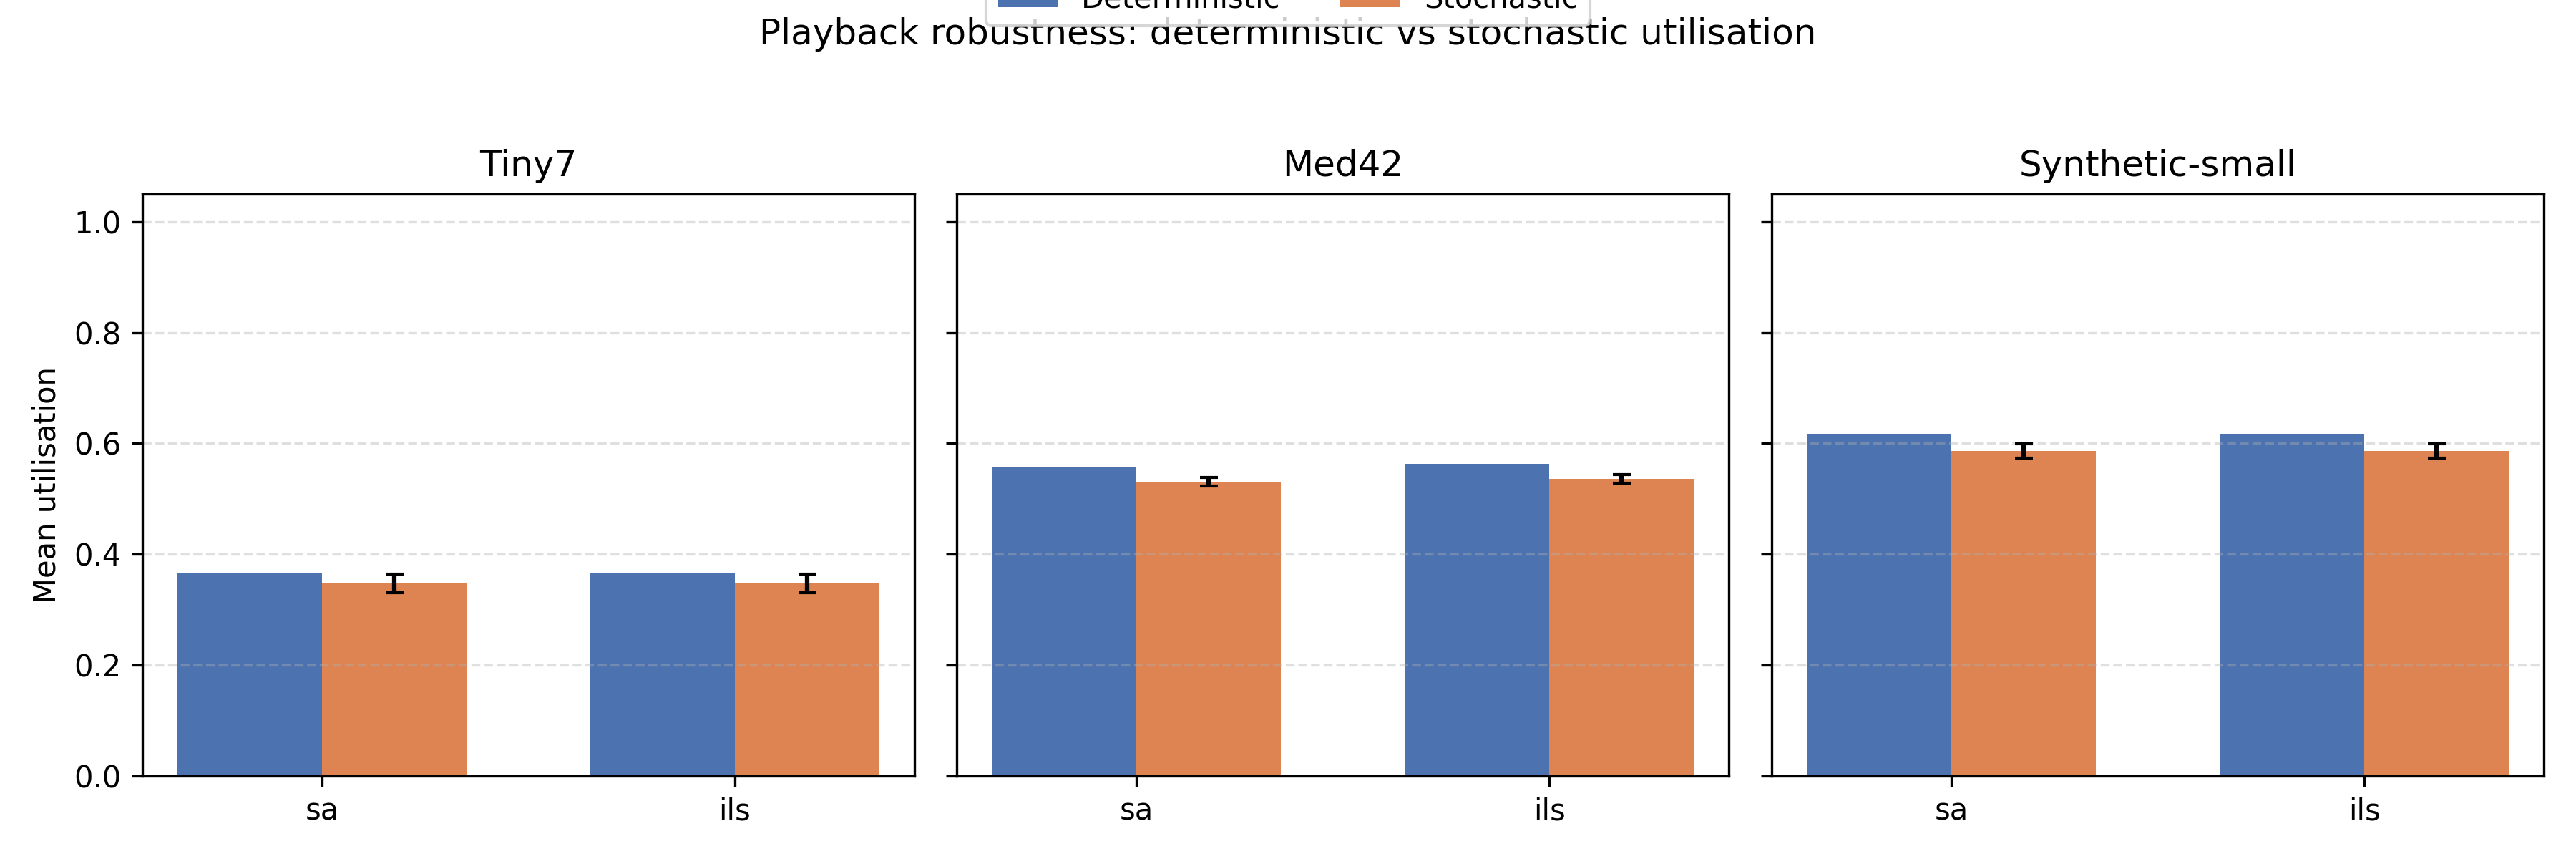
\includegraphics[width=\linewidth]{sections/includes/utilisation_robustness.png}
  \caption{Deterministic vs. stochastic utilization across scenarios. Points denote mean day-level utilization and error bars denote standard deviation over stochastic samples.}
  \label{fig:playback}
\end{figure}

\subsection{Operational question 3: cost interpretation and scaling behavior}
Cost summaries complement utilization and production metrics by translating schedule effects into operating implications. On med42, mobilisation cost in Table~\ref{tab:benchmarks} spans 9846.12--10662.28~CAD across solver choices, indicating that comparable schedule quality can imply different movement-cost profiles. In this baseline, costing is used for within-study comparison, not external economic extrapolation.

Scaling results from synthetic tiers (Figure~\ref{fig:scaling}) show increasing runtime under fixed solver budgets: 31.81~s (small, 4 blocks), 84.88~s (medium, 8 blocks), and 108.97~s (large, 16 blocks). The value is a reproducible scale signal measured in the same platform used for benchmark and robustness reporting.

\begin{figure}[t]
  \centering
  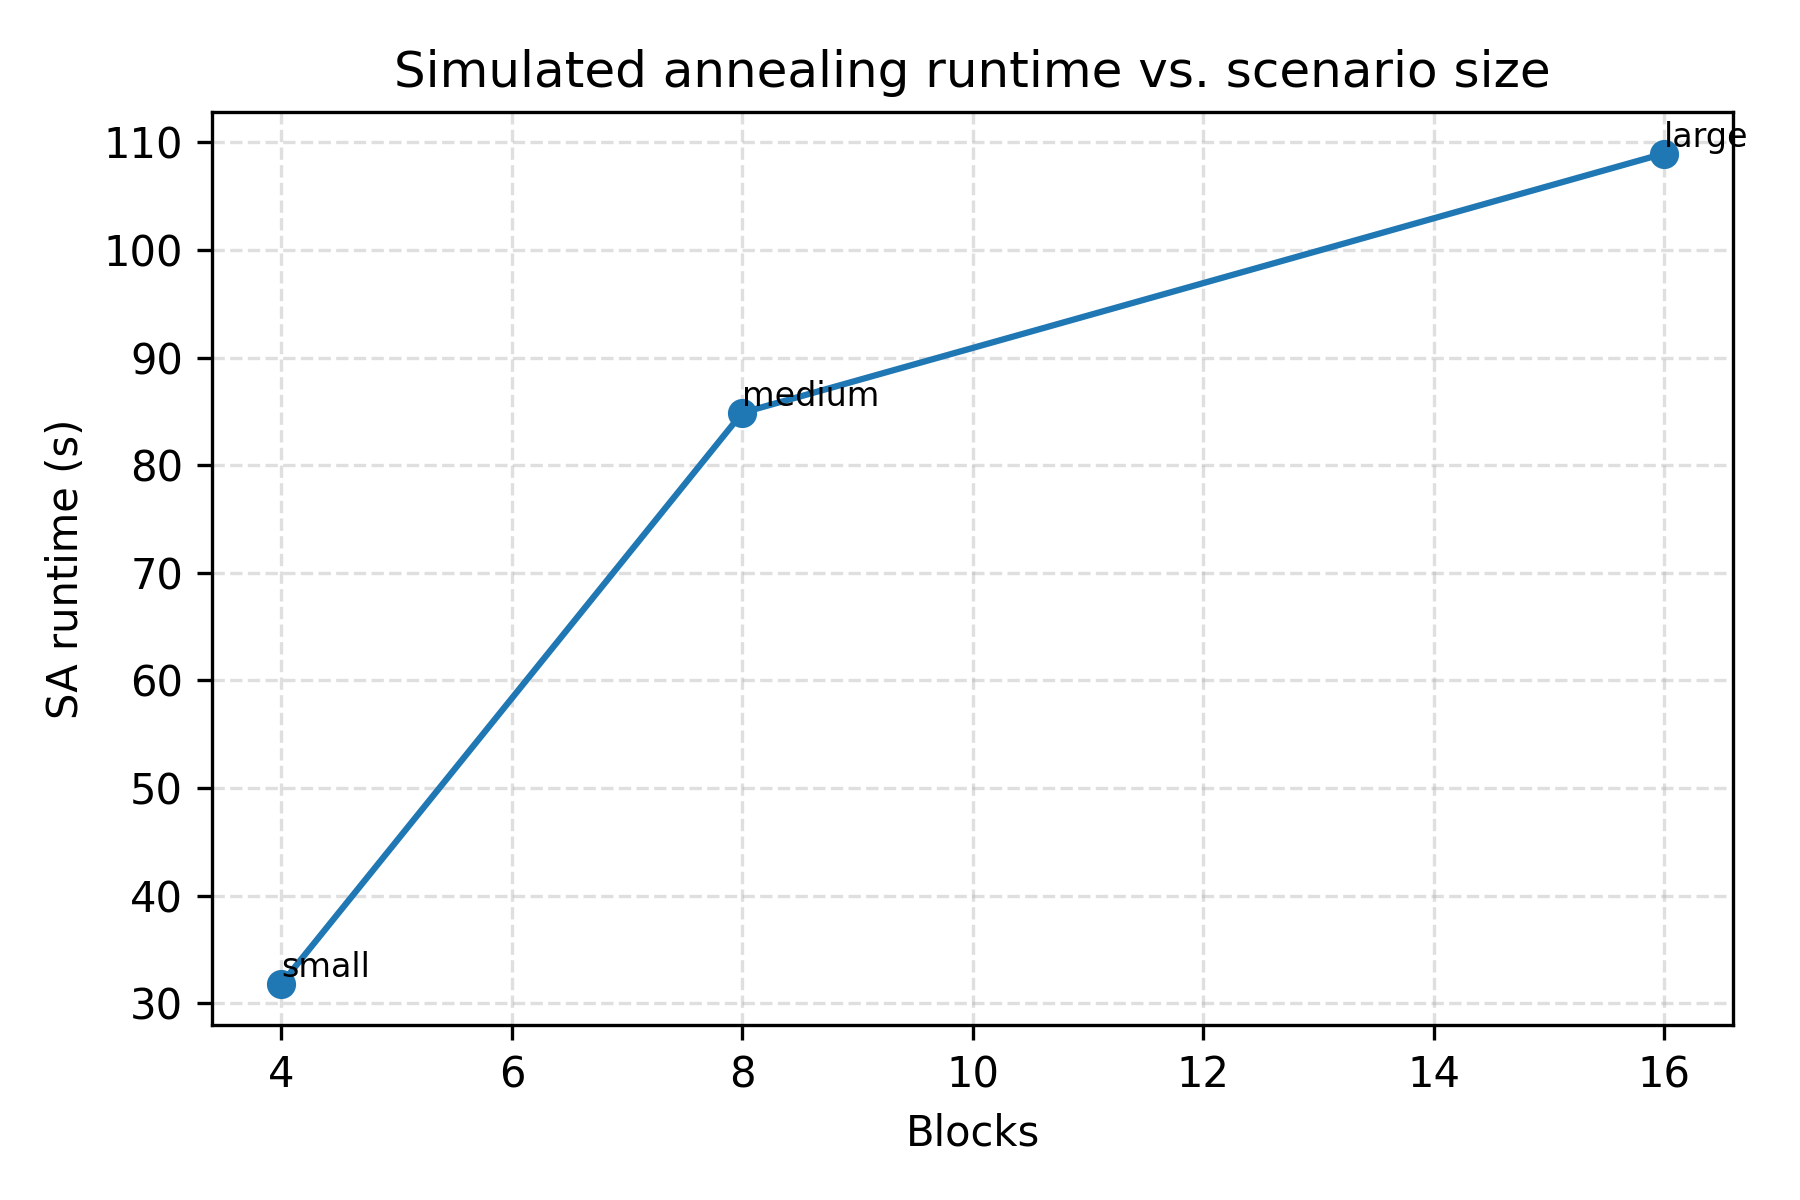
\includegraphics[width=0.8\linewidth]{sections/includes/runtime_vs_blocks.png}
  \caption{Simulated annealing runtime versus number of blocks for synthetic tiers (small, medium, large).}
  \label{fig:scaling}
\end{figure}

\subsection{Scope boundaries and interpretation limits}
Three limits are essential for correct use of this section:
\begin{itemize}
  \item The public ladder currently represents one BC ground-based archetype; broader system families remain out of scope here.
  \item Objective values are comparable within scenario only; cross-scenario interpretation should rely on secondary KPIs (e.g., production, utilization, cost) and relative trends.
  \item Absolute runtime depends on hardware and solver budgets; comparisons in this manuscript are most reliable as within-study baselines.
\end{itemize}

\subsection{Provenance notes}
All tables and figures in this section are generated from versioned manuscript assets and linked run logs so readers can audit values and reuse the same baseline in companion modelling analyses.
